\documentclass[UTF8,oneside]{ctexbook}

\usepackage[titles]{tocloft} % 目录
\usepackage{graphicx} % figure浮动体
\usepackage{animate} % 动画
\usepackage[caption=true, font=footnotesize]{subfig}% 前面的[]为了防止覆盖IEEE默认选项

\usepackage{float} %禁止浮动
\usepackage{enumerate} % 列表

\usepackage{amsmath} % 数学

\usepackage{listings} %抄录环境
\usepackage{color} %定义颜色
\definecolor{codegreen}{rgb}{0,0.6,0}
\definecolor{codegray}{rgb}{0.5,0.5,0.5}
\definecolor{codepurple}{rgb}{0.58,0,0.82}
\definecolor{backcolour}{rgb}{0.95,0.95,0.92}

\definecolor{commentcolor}{rgb}{0.85, 0.85, 0.85}
\definecolor{keywordcolor}{rgb}{0.067, 0.004, 1}
\definecolor{stringcolor}{rgb}{0,0.6,0}
\definecolor{packagecolor}{rgb}{0,0.6,0}
\definecolor{envicolor}{rgb}{0,0.6,0}
%--------- 定义代码抄录格式 -------
\lstdefinestyle{myLaTeX}{
	language={[LaTeX]TeX},
	basicstyle=\small\ttfamily,
	backgroundcolor=\color{backcolour},
	commentstyle=\color{codegreen},
	keywordstyle=\color{magenta},
	numberstyle=\tiny\color{codegray},
	stringstyle=\color{codepurple},
	basicstyle=\footnotesize,
	%
	breakatwhitespace=false,
	breaklines=true, % 允许断行                 
	captionpos=b,
	keepspaces=true,
	numbers=none,numbersep=5pt,
	showspaces=false,
	showstringspaces=false,
	showtabs=false,
	tabsize=2,
	%
	classoffset=1,morekeywords={ctexbook},keywordstyle=\color{keywordcolor}, % classoffest=0为更改默认值
}
\usepackage[colorlinks,linkcolor=blue]{hyperref} % 超链接
\usepackage[margin=3cm]{geometry} % 更改页边距

\usepackage{tcolorbox} % 用于生成彩色文本框
\tcbuselibrary{listings,skins,breakable} %调用程序库
\newtcblisting{mybox}[2][]{colback=black!10!white,colframe=blue!75!black,fonttitle=\bfseries,title=#2,#1,breakable,bicolor,colbacklower=white,% 运行结果部分颜色
interior style={left color=yellow!90,right color=green!40},
frame style={left color=red!75!black,right color=blue!75!black},%哪个[]里有数,证明哪个是必填参数
listing options={
	style=tcblatex,keywordstyle=\color{blue},commentstyle=\color{green!50!black},numbers=none,numberstyle=\tiny\color{red!75!black}\emptyaccsupp,emptylines=1,escapeinside=
	}
}
\usepackage{booktabs} % 用于生成三线表
\usepackage{multirow} % 多行
\usepackage{array}

\title{{\LaTeX 宏包、指令与结果}\\
\large{V1.0}}
\author{\href{https://github.com/lonelybag?tab=repositories}{\itshape{@LonelyBag}}\\ {\itshape \large{Edite by \href{https://mirrors.tuna.tsinghua.edu.cn/CTAN/systems/texlive/Images/}{\LaTeX}}}}

\begin{document}
% ----------- 封面 ---------------
\frontmatter
\maketitle
% ----------- 目录 ---------------
\tableofcontents
\mainmatter
% ----------- 正文 ---------------
\chapter{环境}
% \iffalse \section{========= 不编译 开 =========}
% \section{========= 不编译 关 =========}\fi
% \section{========= 结束 =========}\end{document}
\section{英文环境}
\begin{mybox}[listing only]{\LaTeX 英文环境设置}
\documentclass[journal]{IEEEtran}
\end{mybox}

\section{中文环境}
采用ctex宏集即可,支持的文档类有ctexart、ctexrep、ctexbook 和 ctexbeamer。
\begin{mybox}[listing only]{\LaTeX 中文环境设置}
\documentclass[UTF8,oneside]{ctexbook} % 本书的设置,单列输出
\begin{document}
你可以使用 XeLaTeX、LuaLaTeX 或 upLaTeX 编译,也可以使用 (pdf)LaTeX 编译。
推荐使用 XeLaTeX 或 LuaLaTeX 编译。
\end{document}
\end{mybox}

\section{手动安装宏包}
12
\section{latex转word}
\begin{itemize}
  \item pandoc、\href{https://zhuanlan.zhihu.com/p/43285080}{知乎回答1}
  \item pdf转word
\end{itemize}
\chapter{常用指令}
\section{文档}
\subsection{附录}
\begin{mybox}[listing only]{附录设置}
\appendix
\chapter{附录一}
\end{mybox}

\subsection{设置页边距}
\begin{mybox}[listing only]{更改页边距}
\usepackage[margin=3cm]{geometry} % 更改页边距
\end{mybox}

\subsection{超链接}
\begin{mybox}[]{超链接}
% 宏包:\usepackage{hyperref}
\href{https://github.com/lonelybag/Latex_lonelybag}{Lonelybag的GitHub}
\end{mybox}

\subsection{标尺盒子}
\begin{mybox}[]{标尺盒子}
% 无宏包
% 用法:\rule[raise]{width}{thickness}
\begin{tabular}{|c|}
    \hline
    \rule[-1em]{1em}{1ex}下沉当前字号下M的宽度 \\
    \hline
    \rule[-7pt]{1pt}{28pt}下沉7磅       \\
    \hline
    无支撑                              \\
    \hline
\end{tabular}
\end{mybox}

\subsection{抄录}
\begin{mybox}[]{简单抄录}
% \usepackage{listings} %抄录环境
% 必须预先定义抄录格式
\lstdefinestyle{myLaTeX}{
language={[LaTeX]TeX}, % 继承LaTeX的默认样式
basicstyle=\small\ttfamily,
backgroundcolor=\color{backcolour},
commentstyle=\color{codegreen},
keywordstyle=\color{magenta},
numberstyle=\tiny\color{codegray},
stringstyle=\color{codepurple},
basicstyle=\footnotesize,
% 
breakatwhitespace=false,
breaklines=true, % 允许断行                 
captionpos=b,
keepspaces=true,
numbers=none,numbersep=5pt,
showspaces=false,
showstringspaces=false,
showtabs=false,
tabsize=2,
%
classoffset=1,morekeywords={ctexbook},keywordstyle=\color{keywordcolor},% classoffest=0为更改默认值
}
% 必须定义颜色
% \usepackage{color} %定义颜色
\definecolor{codegreen}{rgb}{0,0.6,0}
\definecolor{codegray}{rgb}{0.5,0.5,0.5}
\definecolor{codepurple}{rgb}{0.58,0,0.82}
\definecolor{backcolour}{rgb}{0.95,0.95,0.92}

\definecolor{commentcolor}{rgb}{0.85, 0.85, 0.85}
\definecolor{keywordcolor}{rgb}{0.067, 0.004, 1}
\definecolor{stringcolor}{rgb}{0,0.6,0}
\definecolor{packagecolor}{rgb}{0,0.6,0}
\definecolor{envicolor}{rgb}{0,0.6,0}

\begin{lstlisting}[style=myLaTeX,frame=single]
这是抄录内容,比如\usepackage{tcolorbox}
\end{lstlisting}
\end{mybox}

\subsection{复杂抄录}
\begin{mybox}[listing only]{复杂抄录}
% 宏包:\usepackage{tcolorbox} % 用于生成彩色文本框
\tcbuselibrary{listings,skins,breakable} %调用程序库
\newtcblisting{mybox}[2][]{
 colback=red!5!white,
 colframe=red!75!black,
 fonttitle=\bfseries,
 title=#2,#1,
 breakable,
 bicolor,colbacklower=white,interior style={left color=yellow!70,right color=green!70},%哪个[]里有数,证明哪个是必填参数
 listing options={
  style=tcblatex,
  keywordstyle=\color{blue},
  commentstyle=\color{green!50!black},
  numbers=none,
  numberstyle=\tiny\color{red!75!black}\emptyaccsupp,
  emptylines=1,
  escapeinside=}
}
\end{mybox}

\begin{lstlisting}[style=myLaTeX,frame=single]
	\begin{mybox}[listing only]{这里放标题}
		复杂抄录
	\end{mybox}
\end{lstlisting}

\section{表格}
\noindent 参考:\href{http://www.latexstudio.net/archives/9842.html}{\LaTeX 中文论坛}
\subsection{三线表}
\begin{mybox}[]{三线表}
% \usepackage{booktabs} % 用于生成三线表

\begin{tabular}{cccc}
\toprule
               & \multicolumn{3}{c}{Numbers} \\
  \cmidrule{2-4}
               & 1 & 2 & 3                   \\
  \midrule
  Alphabet     & A & B & C                   \\
  Roman        & I & II& III                 \\
  \bottomrule
\end{tabular}
\end{mybox}

\subsection{合并行列}

\begin{mybox}[]{原始}
%\usepackage{multirow}
  
%\begin{table*}[!hbt]
%\centering
%\caption{表格}\label{tab:2}
%\vspace{-0.2cm}

%\renewcommand{\arraystretch}{1.3} %可以让行显得更加宽敞
%\resizebox{\textwidth}{12mm}{  % 原表格过宽,调节高度,宽度为该环境下行宽
%\resizebox{\linewidth}{!}{  % 原表格过宽,调节宽度
%\setlength{\tabcolsep}{1mm}{ % 原表格过窄

  \begin{tabular}{|c|c|c|c|}
  \hline
  \multicolumn{4}{|c|}{总标题}                                \\ % 注意:每行填充完毕后,必须回车
  \hline
  \multicolumn{2}{|c|}{类型}& 第三列 & 第四列                  \\
  \hline
  \multirow{2}{*}{合并两行1}& A & A1 & \multirow{2}{*}{numbers}\\
  \cline{2-3}  % 换行后,绘制上表格底边, 且格式必须为 ‘A-B’
                            & B & B1 &                         \\
  \cline{1-4}
  \multirow{2}{*}{合并两行2}& C & C1 & \multirow{2}{*}{numbers}\\
  \cline{2-3}
                            & D & D1 &                         \\
  \hline
  \end{tabular}
%}
%\end{table*}
\end{mybox}

\begin{mybox}[]{合并行列}
% \usepackage{multirow}

\renewcommand{\arraystretch}{1} %可以让行显得更加宽敞
%\resizebox{\textwidth}{12mm}{  % 原表格过宽,调节高度,宽度为该环境下行宽
%\resizebox{\linewidth}{!}{  % 原表格过宽,调节宽度
\setlength{\tabcolsep}{10mm}{ % 原表格过窄
\begin{tabular}{|c|c|c|c|}
\hline
\multicolumn{4}{|c|}{总标题}                                \\ % 注意:每行填充完毕后,必须回车
\hline
\multicolumn{2}{|c|}{类型}& 第三列 & 第四列                  \\
\hline
\multirow{2}{*}{合并两行1}& A & A1 & \multirow{2}{*}{numbers}\\
\cline{2-3}  % 换行后,绘制上表格底边, 且格式必须为 ‘A-B’
                          & B & B1 &                         \\
\cline{1-4}
\multirow{2}{*}{合并两行2}& C & C1 & \multirow{2}{*}{numbers}\\
\cline{2-3}
                          & D & D1 &                         \\
\hline
\end{tabular}
}
%\vspace{5cm}% 可以控制空白区域的大小
\end{mybox}

\begin{mybox}[]{调节字体大小}
  % \usepackage{multirow}
  % \usepackage{array} % 调节字体大小
  
  \renewcommand{\arraystretch}{1} %可以让行显得更加宽敞
  %\resizebox{\textwidth}{12mm}{  % 原表格过宽,调节高度,宽度为该环境下行宽
  %\resizebox{\linewidth}{!}{  % 原表格过宽,调节宽度
  %\setlength{\tabcolsep}{10mm}{ % 原表格过窄
  \begin{tabular}{|>{\huge}c|c|c|c|}
  \hline
  \multicolumn{4}{|c|}{总标题}                                \\ % 注意:每行填充完毕后,必须回车
  \hline
  \multicolumn{2}{|c|}{类型}& 第三列 & 第四列                  \\
  \hline
  \multirow{2}{*}{合并两行1}& A & A1 & \multirow{2}{*}{numbers}\\
  \cline{2-3}  % 换行后,绘制上表格底边, 且格式必须为 ‘A-B’
                            & B & B1 &                         \\
  \cline{1-4}
  \multirow{2}{*}{合并两行2}& C & C1 & \multirow{2}{*}{numbers}\\
  \cline{2-3}
                            & D & D1 &                         \\
  \hline
  \end{tabular}
  %}
  \end{mybox}


\subsection{表格绘制工具}
\begin{itemize}
  \item \href{https://www.tablesgenerator.com/#}{在线绘制表格}
  \item \href{http://www.latexstudio.net/archives/6992.html}{Excel插件:Excel2LaTeX}
\end{itemize}

\section{插图}
\subsection{一张图}
\begin{mybox}[]{一张图}
% \usepackage{graphicx} % figure浮动体
% \usepackage{float} %禁止浮动

\begin{figure}[H]
  \centering
  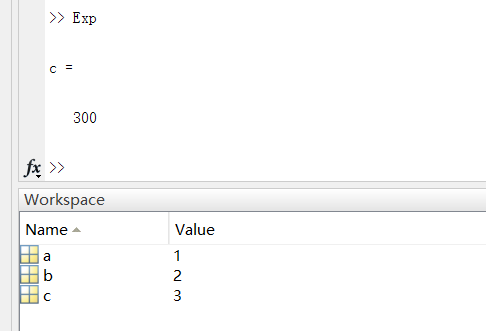
\includegraphics[width=0.3\linewidth]{Fig//base_workspace.png}
  \vspace{-0.3cm}
  \caption{函数脚本 - base workspace}\label{fig:base_workspace}
\end{figure}
\end{mybox}


\subsection{1列}
\begin{mybox}[]{1列}
% \usepackage[caption=true, font=footnotesize]{subfig}% 前面的[]为了防止覆盖IEEE默认选项
% \usepackage{graphicx} % figure浮动体
% \usepackage{float} %禁止浮动

\begin{figure}[H]
\centering
\subfloat[设置模型回调函数]{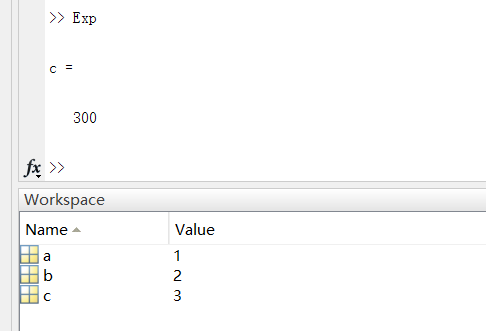
\includegraphics[width=0.3\linewidth]{Fig//base_workspace.png}}\\ % []中括号写标注
\vspace{-0.4cm}
\subfloat[设置初始回调函数]{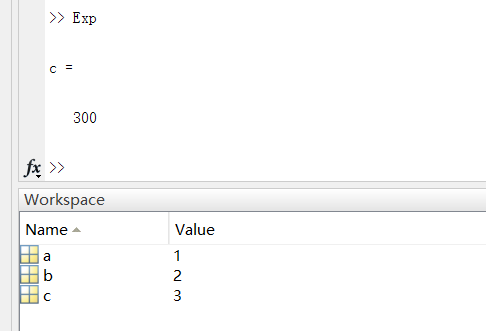
\includegraphics[width=0.3\linewidth]{Fig//base_workspace.png}}
\vspace{-0.2cm}
\caption{回调函数设置}\label{fig:callbacksetup}
\vspace{-0.5cm}
\end{figure}
\end{mybox}

\subsection{2行2列}
\begin{mybox}[]{2行2列}
% \usepackage[caption=true, font=footnotesize]{subfig}% 前面的[]为了防止覆盖IEEE默认选项
% \usepackage{graphicx} % figure浮动体
% \usepackage{float} %禁止浮动

\begin{figure}[H]
  \begin{minipage}{0.48\linewidth}
    \centerline{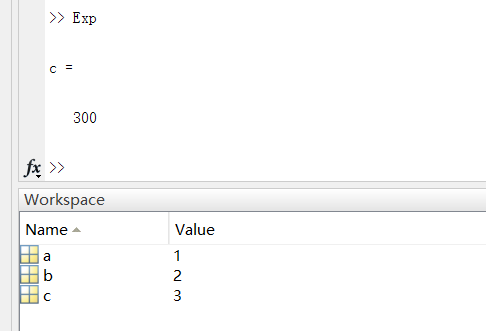
\includegraphics[width=4.0cm]{Fig//base_workspace.png}}
    \centerline{(a)}
  \end{minipage}
  \hfill
  \begin{minipage}{.48\linewidth}
    \centerline{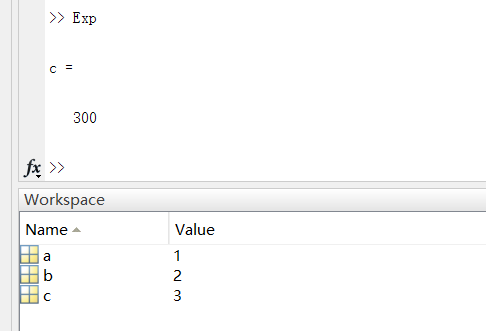
\includegraphics[width=4.0cm]{Fig//base_workspace.png}}
    \centerline{(b)}
  \end{minipage}
  \vfill
  \begin{minipage}{0.48\linewidth}
    \centerline{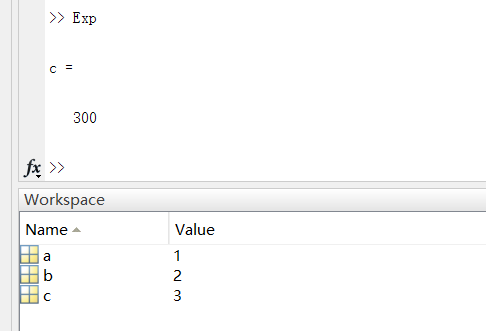
\includegraphics[width=4.0cm]{Fig//base_workspace.png}}
    \centerline{(c)}
  \end{minipage}
  \hfill
  \begin{minipage}{0.48\linewidth}
    \centerline{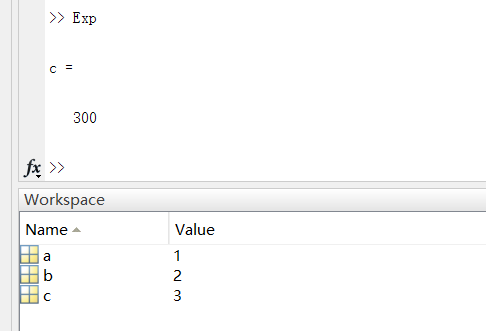
\includegraphics[width=4.0cm]{Fig//base_workspace.png}}
    \centerline{(d)}
  \end{minipage}
  \caption{2$\times$2}\label{fig:res}
  \end{figure}
\end{mybox}


\begin{mybox}[]{按列分组排列}
% \usepackage[caption=true, font=footnotesize]{subfig}% 前面的[]为了防止覆盖IEEE默认选项
% \usepackage{graphicx} % figure浮动体
% \usepackage{float} %禁止浮动

\begin{figure}[H]
  \centering
  \subfloat[第一列]{
  \begin{minipage}[b]{0.23\linewidth}
    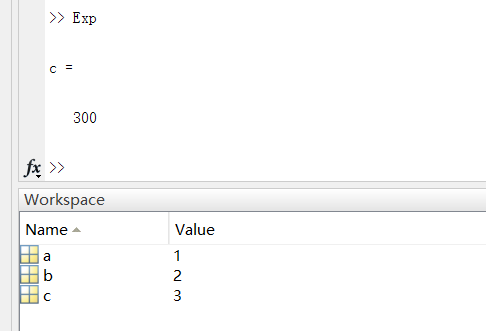
\includegraphics[width=1\linewidth]{Fig//base_workspace.png}\vspace{4pt}
    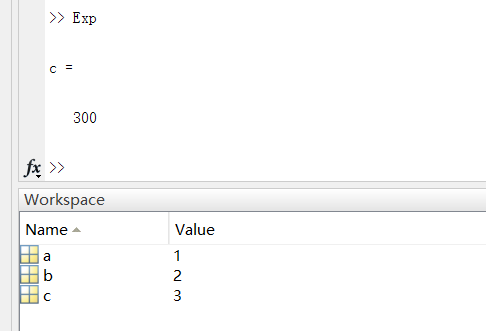
\includegraphics[width=1\linewidth]{Fig//base_workspace.png}\vspace{4pt}
    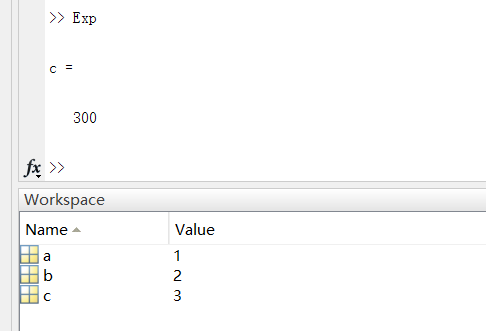
\includegraphics[width=1\linewidth]{Fig//base_workspace.png}\vspace{4pt}
    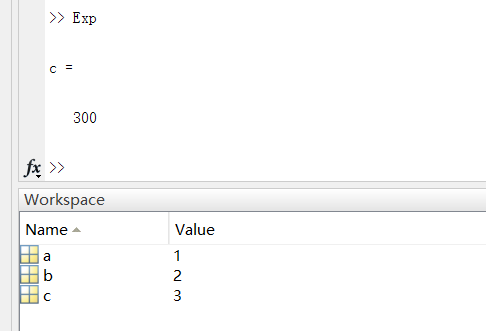
\includegraphics[width=1\linewidth]{Fig//base_workspace.png}
  \end{minipage}}
  \subfloat[第二列]{
  \begin{minipage}[b]{0.23\linewidth}
    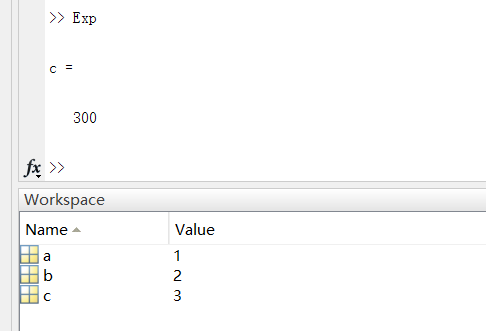
\includegraphics[width=1\linewidth]{Fig//base_workspace.png}\vspace{4pt}
    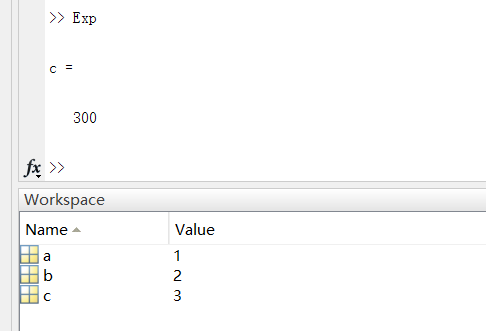
\includegraphics[width=1\linewidth]{Fig//base_workspace.png}\vspace{4pt}
    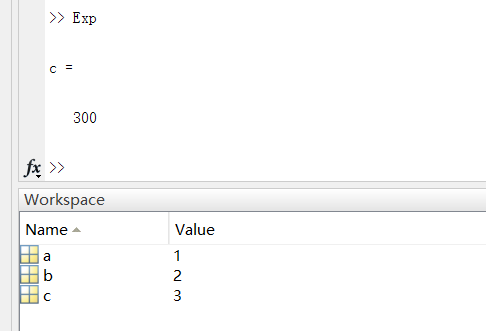
\includegraphics[width=1\linewidth]{Fig//base_workspace.png}\vspace{4pt}
    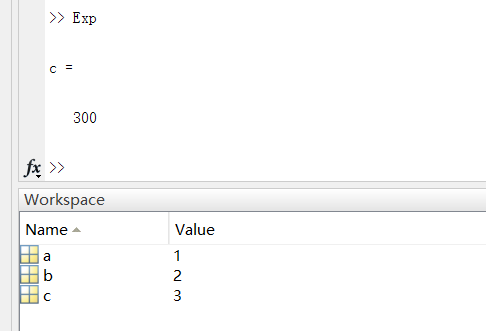
\includegraphics[width=1\linewidth]{Fig//base_workspace.png}
  \end{minipage}}
  \subfloat[第三列]{
  \begin{minipage}[b]{0.23\linewidth}
    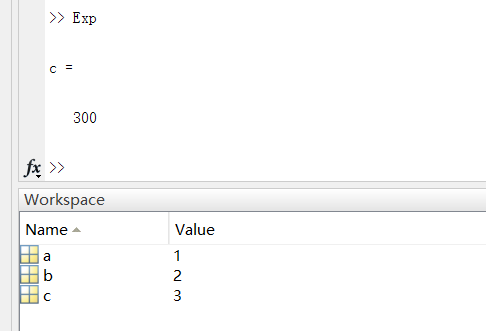
\includegraphics[width=1\linewidth]{Fig//base_workspace.png}\vspace{4pt}
    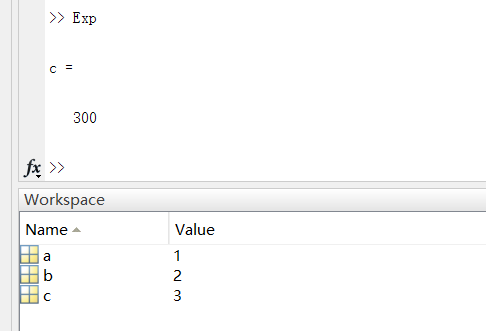
\includegraphics[width=1\linewidth]{Fig//base_workspace.png}\vspace{4pt}
    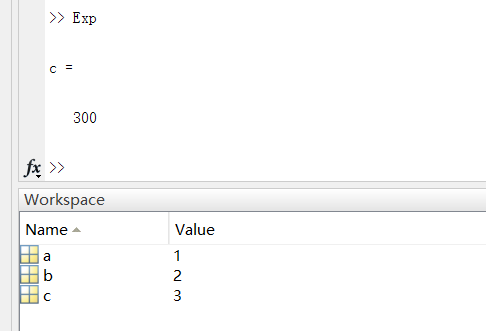
\includegraphics[width=1\linewidth]{Fig//base_workspace.png}\vspace{4pt}
    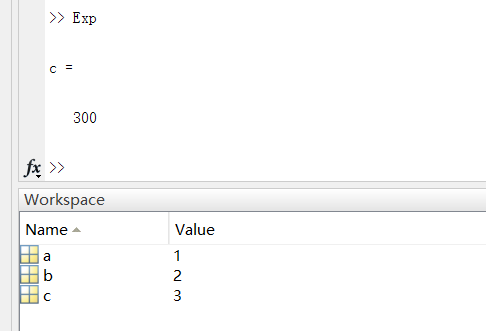
\includegraphics[width=1\linewidth]{Fig//base_workspace.png}
  \end{minipage}}
  \subfloat[第四列]{
  \begin{minipage}[b]{0.23\linewidth}
    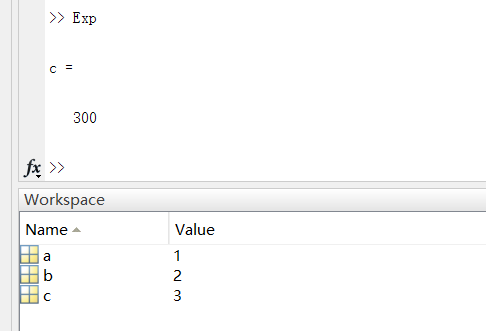
\includegraphics[width=1\linewidth]{Fig//base_workspace.png}\vspace{4pt}
    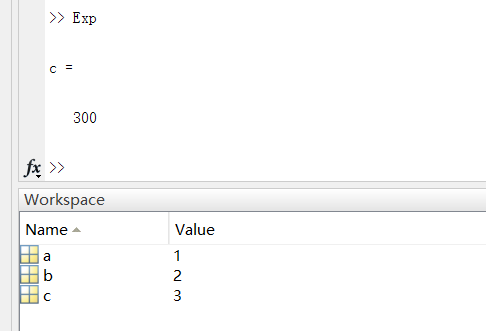
\includegraphics[width=1\linewidth]{Fig//base_workspace.png}\vspace{4pt}
    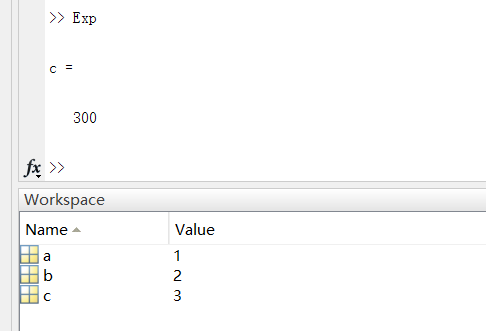
\includegraphics[width=1\linewidth]{Fig//base_workspace.png}\vspace{4pt}
    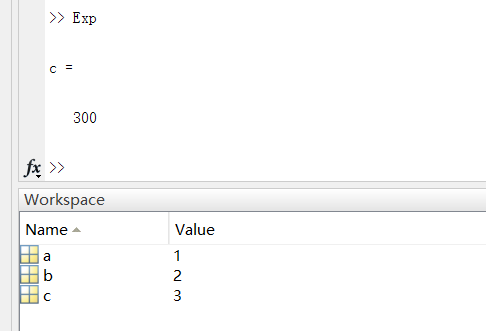
\includegraphics[width=1\linewidth]{Fig//base_workspace.png}
  \end{minipage}}
  \caption{按列排列}
\end{figure}
\end{mybox}

\subsection{动画}
\begin{mybox}[]{动画}
% \usepackage{graphicx} % figure浮动体
% \usepackage{animate} % 动画
% \usepackage{float} % 禁止浮动,可将figure参数设置为H,否则只能是hbt

\begin{figure}[H]
  \centering
  \animategraphics[autoplay, loop , width=0.6\linewidth]{10}{Fig//reflected1//}{1}{10} % 路径必须与tex源文件在同一根目录中
  \vspace{-0.3cm}
  \caption{终端短路}\label{fig:reflected1}
\end{figure}
\end{mybox}




\end{document}